
%  \section{The analysis of FWHM behavior} 

Now that we understand that the seeing is by and large described by 
a single parameter, FWHM, we study three aspects of its variation, as follows.


\subsection{The FWHM dependence on wavelength} 

The Kolmogorov turbulence theory gives a standard formula for the FWHM of a long-exposure
seeing-limited PSF in a large telescope,
\begin{equation}
FWHM^{Kolm}(\lambda, X) = \frac{0.976\lambda}{r_0(\lambda,X)}.
\label{eq:fwhmkolm}
\end{equation}
Here $\lambda$ is the wavelength, and $X$ is the airmass.
We use $\lambda = 500$nm as the reference wavelength,
\begin{equation}
r_0(\lambda,X) = r_0(500) \left(\frac{\lambda}{500}\right)^{1.2}
\frac{1}{X^{0.6}},
\label{eq:r0}
\end{equation}
where $r_0(500)$ is the $r_0$ for $\lambda=500$nm and $X$=1, and $\lambda$ is in
the unit of nm.
Substituting Eq.~(\ref{eq:r0}) into (\ref{eq:fwhmkolm}), it is easy to see
\begin{equation}
FWHM^{Kolm} \propto \lambda^{-0.2}.
\end{equation}


With the von Karman atmosphere model, the FWHM as in
Eq.~(\ref{eq:fwhmkolm}) needs an additional correction factor
which is a function of the outer scale $L_0$~\citep{Tokovinin2002},
\begin{equation}
FWHM^{vonK}(\lambda, X) = \frac{0.976\lambda}{r_0(\lambda,X)}
\sqrt{1-2.183\left( \frac{r_0(\lambda,X) }{L_0} \right)^{0.356}}.
\end{equation}
If we still want to write $FWHM^{vonK} \propto \lambda^{\alpha} $, 
$\alpha$ will be a function of $L_0$ and $r_0$ at a specified
wavelength and airmass, or equivalently, $L_0$ and $FWHM^{vonK}$ at a
specified wavelength and airmass. Below, we will use SDSS 
PSF FWHM measurements from the 
$r$-band,
whose effective wavelength is 616.6 nm, and airmass of 1.
In this work, we always use FWHM to refer to FWHM$^{vonK}$.

For each run from SDSS Stripe 82 data, and each camera column, we make
a least-square fit to
all the simultaneous FWHM measurements across the optical bands, to
estimate the power parameter $\alpha$.
All FWHM are multiplied with $1/X^{0.6}$ to correct for airmass.
We take into account that the same field number doesn't correspond to the same
time in all filters. The scanning order in the SDSS camera is $r$-$i$-$u$-$z$-$g$, with the delay between the two 
successive filters corresponding to 2 fields. That is, If we take the field number $F$ for the $r$-band, then
we need to take FWHM for the $i$-band from field $F-2$, for the u band
from $F-4$, and so on. Fig.~\ref{fig:fwhm_lambda} shows such fits for
run 4874. All FWHM are normalized using corresponding FWHM in the
$r$-band taken at the same moment in time.
Significant deviation from $\alpha = -0.2$, as predicted by the
Kolmogorov model, can be seen in most bands.

\begin{figure}
\centering
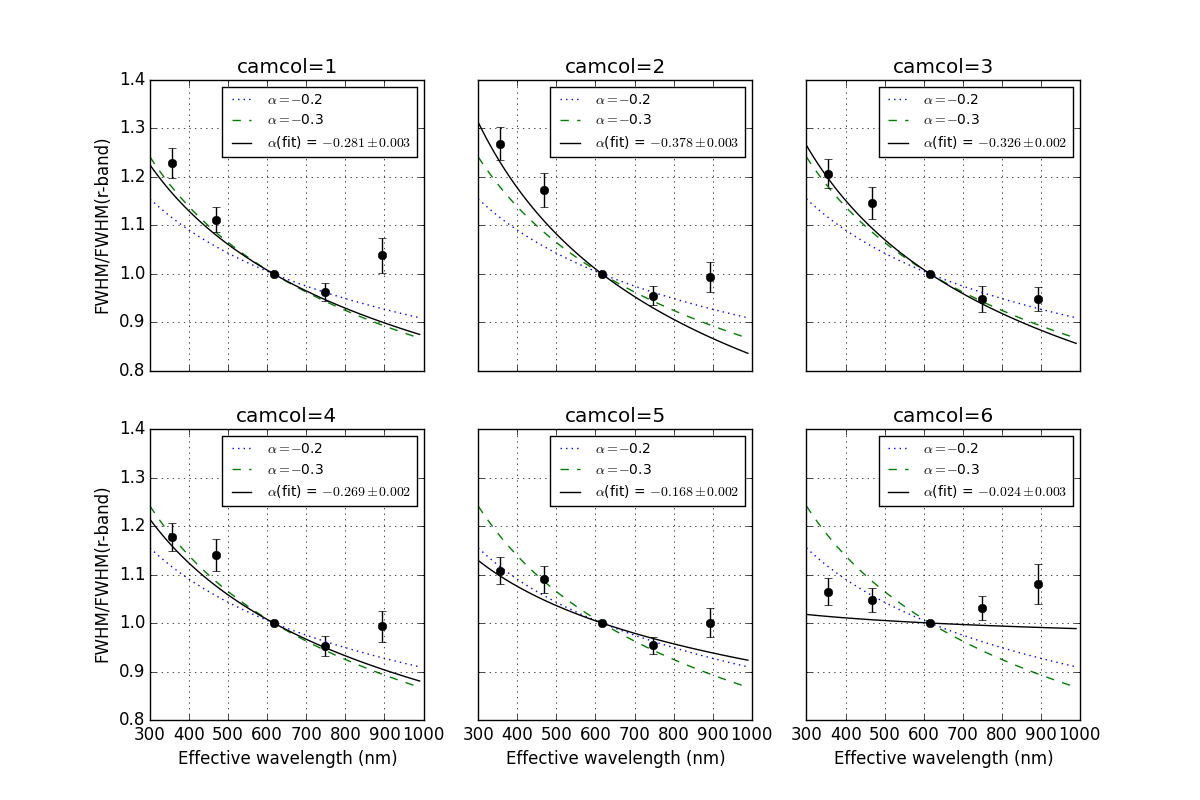
\includegraphics[width=0.9\textwidth]{FIGURES/fwhm_lambda.png}
\caption{FWHM as functions of wavelength for run 4874.
For comparison purposes, the $\alpha=-0.2$ (dotted) and $\alpha=-0.3$ (dashed) lines are
also shown.
\label{fig:fwhm_lambda}}
\end{figure}

As discussed above, based on the von Karman atmosphere model, the
power $\alpha$ should be a function of outer scale $L_0$ and the
FWHM in a specified optical band.
Fig.~\ref{fig:alpha_fwhm} is a scattered plot of $\alpha$ versus FWHM
in the $r$-band, for all the Stripe 82 runs.
A correlation between $\alpha$ and the FWHM seems to be present.
Similar correlations have been seen in Subaru images and reported by~\cite{subaruSeeing2016}.
The data points are overlaid with curves as predicted by the von
Karman model, with varying $L_0$, ranging from 2 meters to infinity.
The data clear deviate from the Kolmogorov model prediction, which is
the horizontal line at $\alpha = -0.20$, with infinite $L_0$.
For LSST, using the commonly assumed $L_0 = 30$m, and a FWHM of 0.6
arcsec, we get a $\alpha$ value close to $-0.30$.

\begin{figure}
\centering
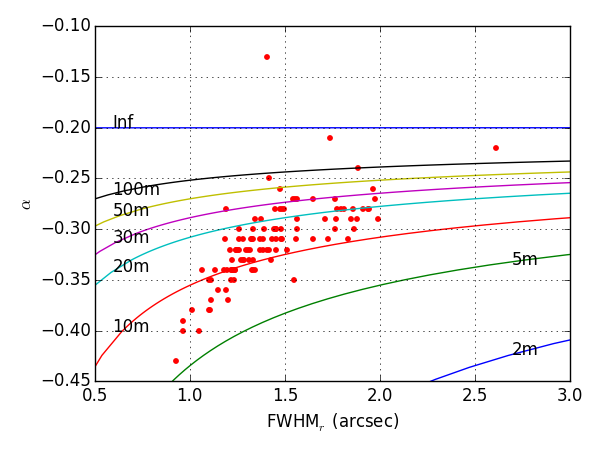
\includegraphics[width=0.5\textwidth]{FIGURES/alpha_fwhm.png}
\caption{Wavelength-dependence power parameter $\alpha$ vs the
  FWHM in the $r$-band for all the Stripe 82 runs. 
The curves are predictions of the von Karman
  model, with $L_0$ ranging from 2 meters to infinity.
\label{fig:alpha_fwhm}}
\end{figure}



\subsection{Angular structure function} 

To examine the spatial correlation of the FWHM we compute the angular
structure function using PSF measurements from all 6 camera columns.
Our structure function is defined as
the root-mean-square of the PSF size differences of pairs of stars
in the same angular bin. 
Results are shown in Fig.~\ref{fig:spatial}.
The SDSS curves are combined for 86 out of the 108 Stripe 82 runs with number of
fields more than 100, then for all
the optical bands. We also checked the structure function for each band
separately, and found no statistically significant difference.

For comparison, Fig. ~\ref{fig:spatial} also shows the PSF angular
structure functions obtained using PhoSim~\citep{phosim} by simulating LSST,
and that from CFHT PSF measurements~\citep{heymans2012}.
The PhoSim PSF profiles are obtained by simulating a grid of stars
spaced by 6 arcminutes with non-perturbed telescope and ideal sensors.
The results are averaged over 9 different atmosphere realizations with
different wind and screen parameters and airmass, and with 3 different
wavelength, 350 nm, 660 nm, and 970 nm.
The CFHT PSF size measurements are provided by Heymans.
The 3 curves in Fig.~\ref{fig:spatial} appear to be quantitatively
consistent with each other, even though they are for different telescopes.


\begin{figure}
\centering
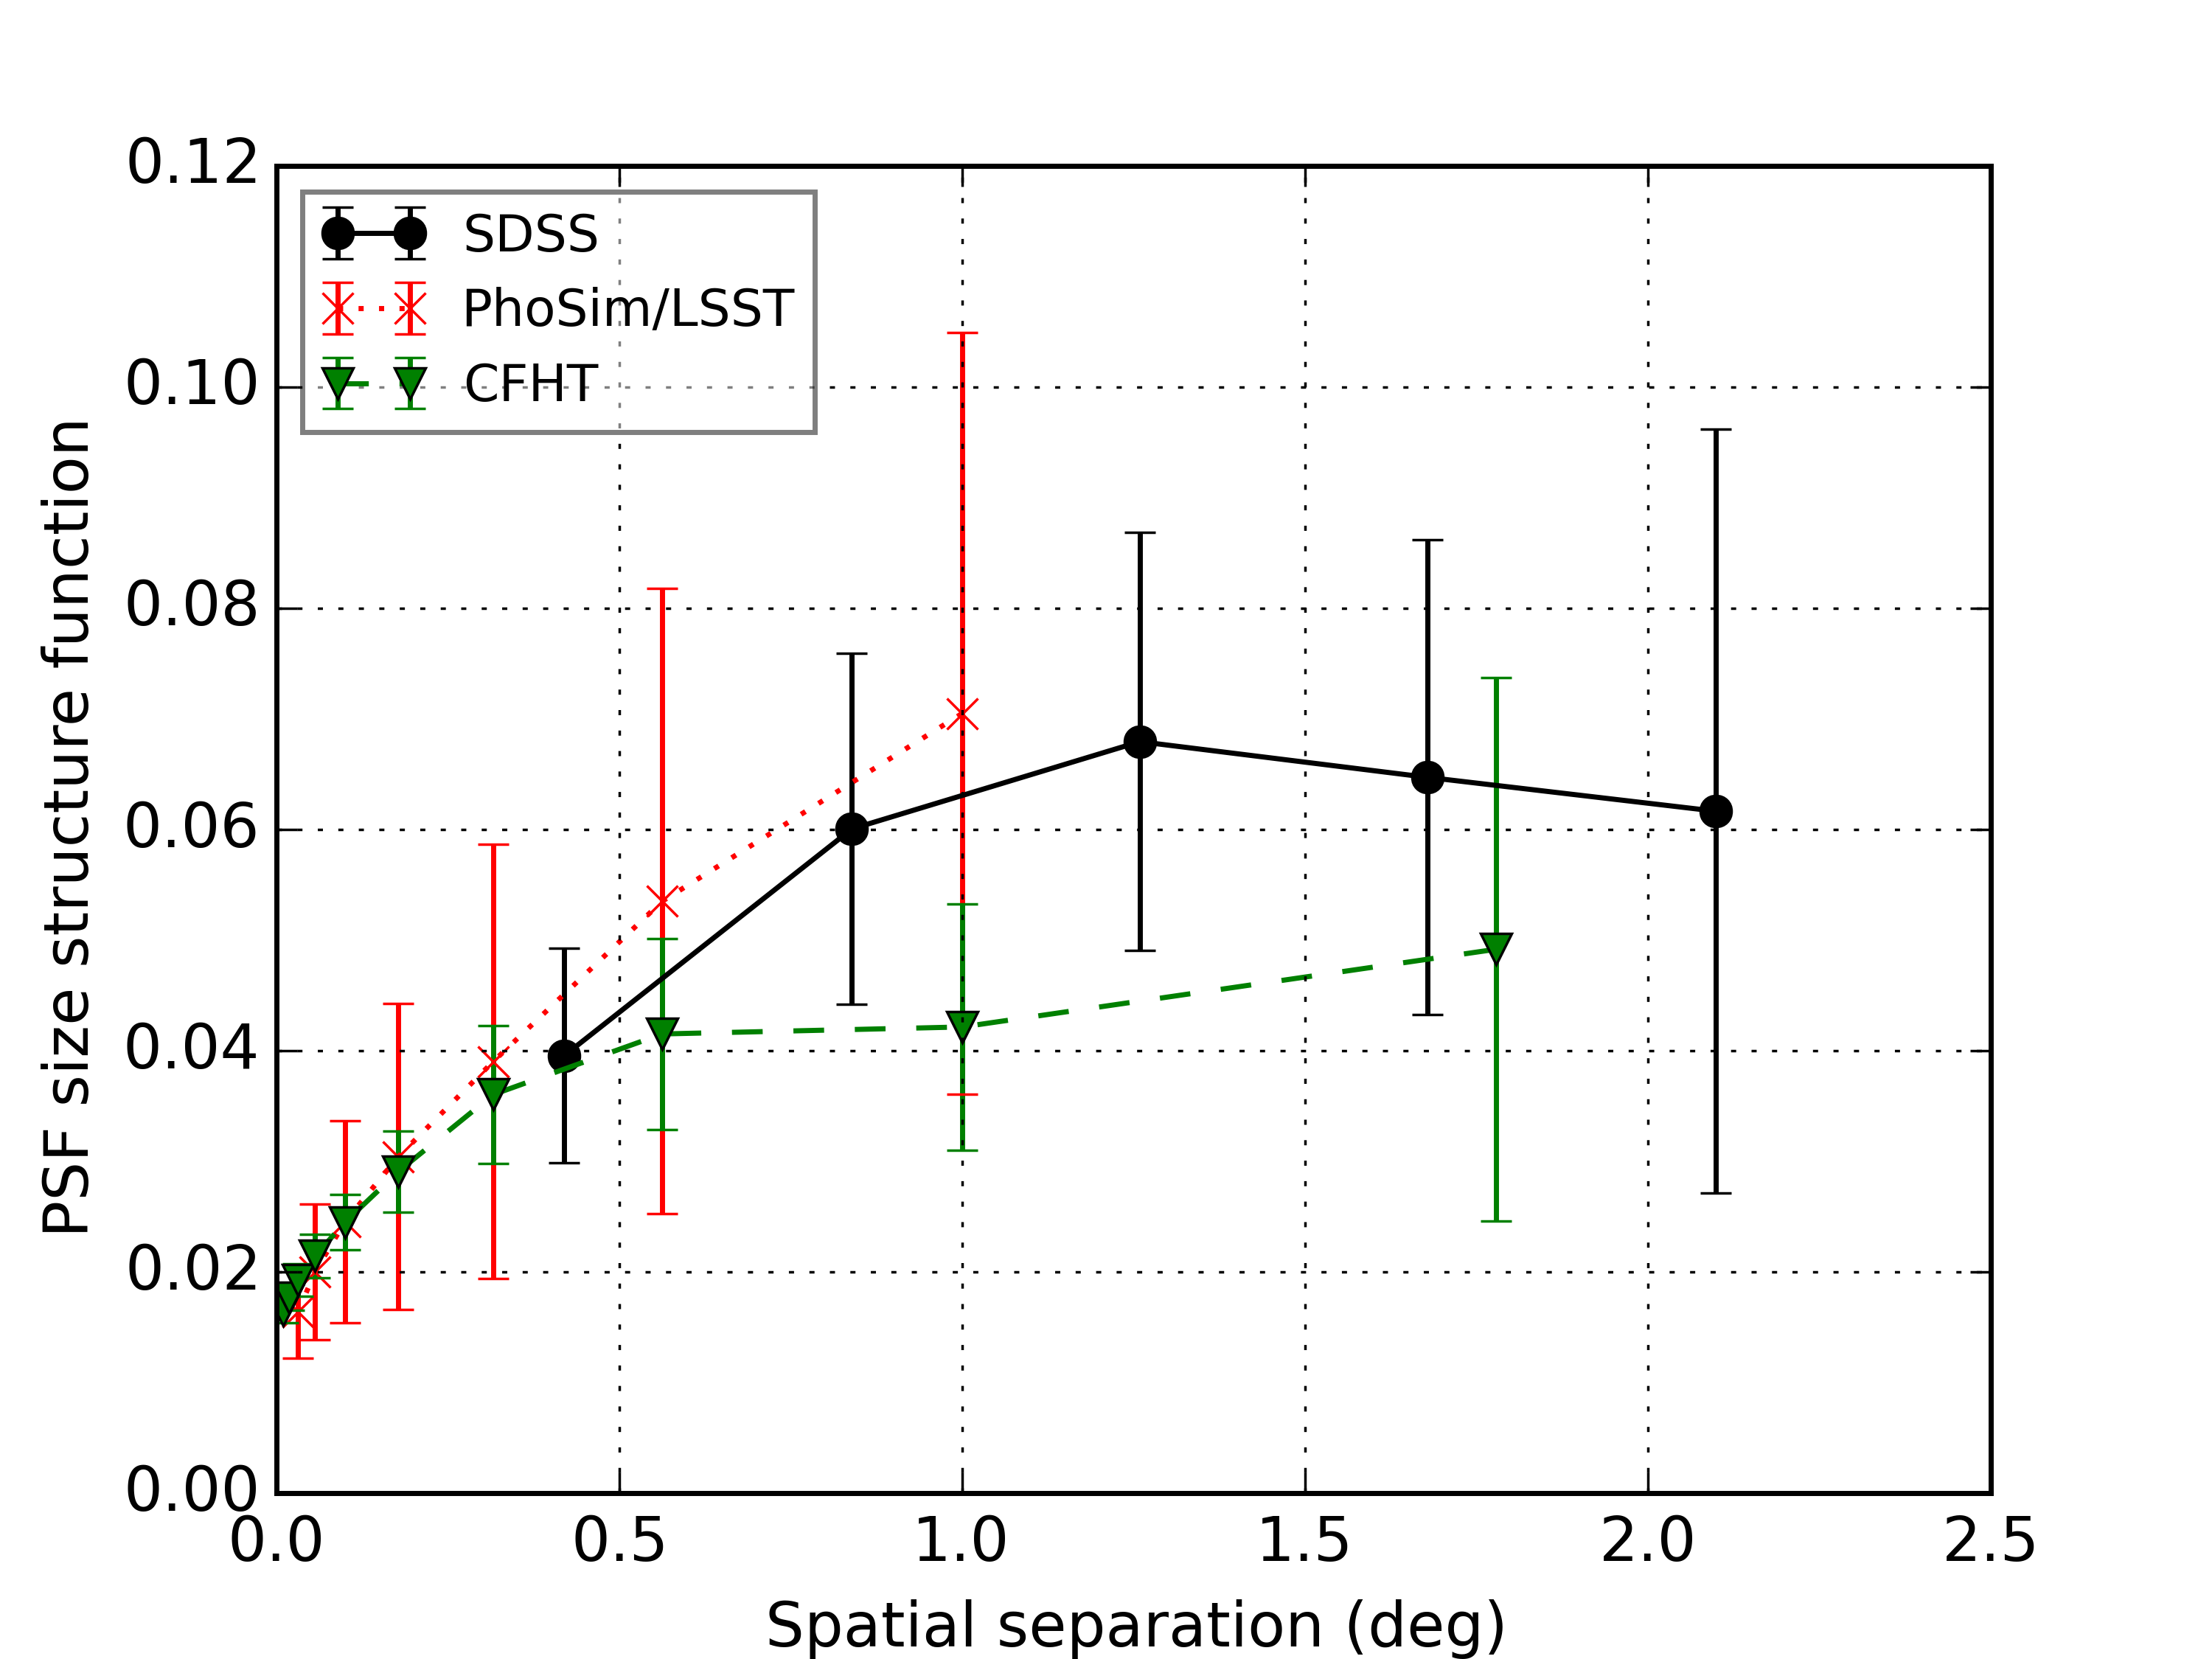
\includegraphics[width=0.5\textwidth]{FIGURES/spatial.png}
\caption{PSF size angular structure function using SDSS measurements
  combined over 86 out of the 108 runs with number of fields larger
  than 100, and comparisons with PhoSim simulations and CFHT
  measurements of the same quantity.
\label{fig:spatial}}
\end{figure}

\subsection{Temporal auto-correlation function}

To study the temporal behavior of the seeing, we look at the 
 power spectrum.
Fig.~\ref{fig:psd} shows the temporal power spectral density (PSD) of the
PSF FWHM for 6 camera columns, in run 4874, $r$-band.
We fit the PSD to the damped random walk model~\citep{zeljkoBook},
\begin{equation}
PSD(f) = \frac{\tau^2 SF^2_{\infty}}{1+(2\pi f \tau)^2},
\end{equation}
where $f$ is the temporal frequency, $SF_{\infty}$ is the asymptotic
value of the structure function, and $\tau$ is the
characteristic timescale.
Combining fit results for all camera columns and optical bands for run 4874
gives $\tau = 15.1 \pm 1.4$ minutes.
This is consistent with ~\cite{Racine1996}, where a timescale of 
$\tau = 17 \pm 1$ minutes was found.
Making the same fits for all the Stripe 82 runs with number of fields
larger than 600, the values of $\tau$ are plotted in Fig.~\ref{fig:hist}.

\begin{figure}
\centering
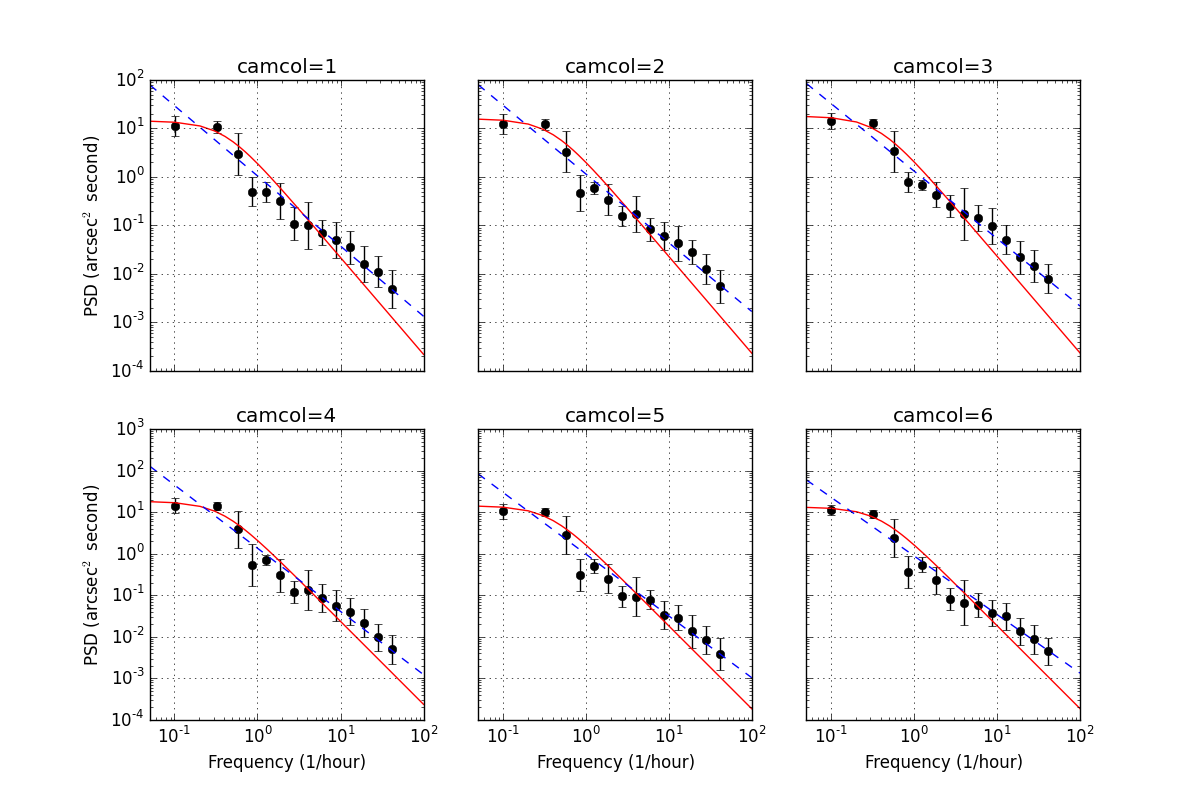
\includegraphics[width=0.9\textwidth]{FIGURES/temporalPSD.png}
\caption{PSF size temporal power spectral density for run 4874, r-band. 
Combining fit results for all camera columns and optical bands for
this run
gives $\tau = 15.1 \pm 1.4$ minutes.
\label{fig:psd}}
\end{figure}

\begin{figure}
\centering
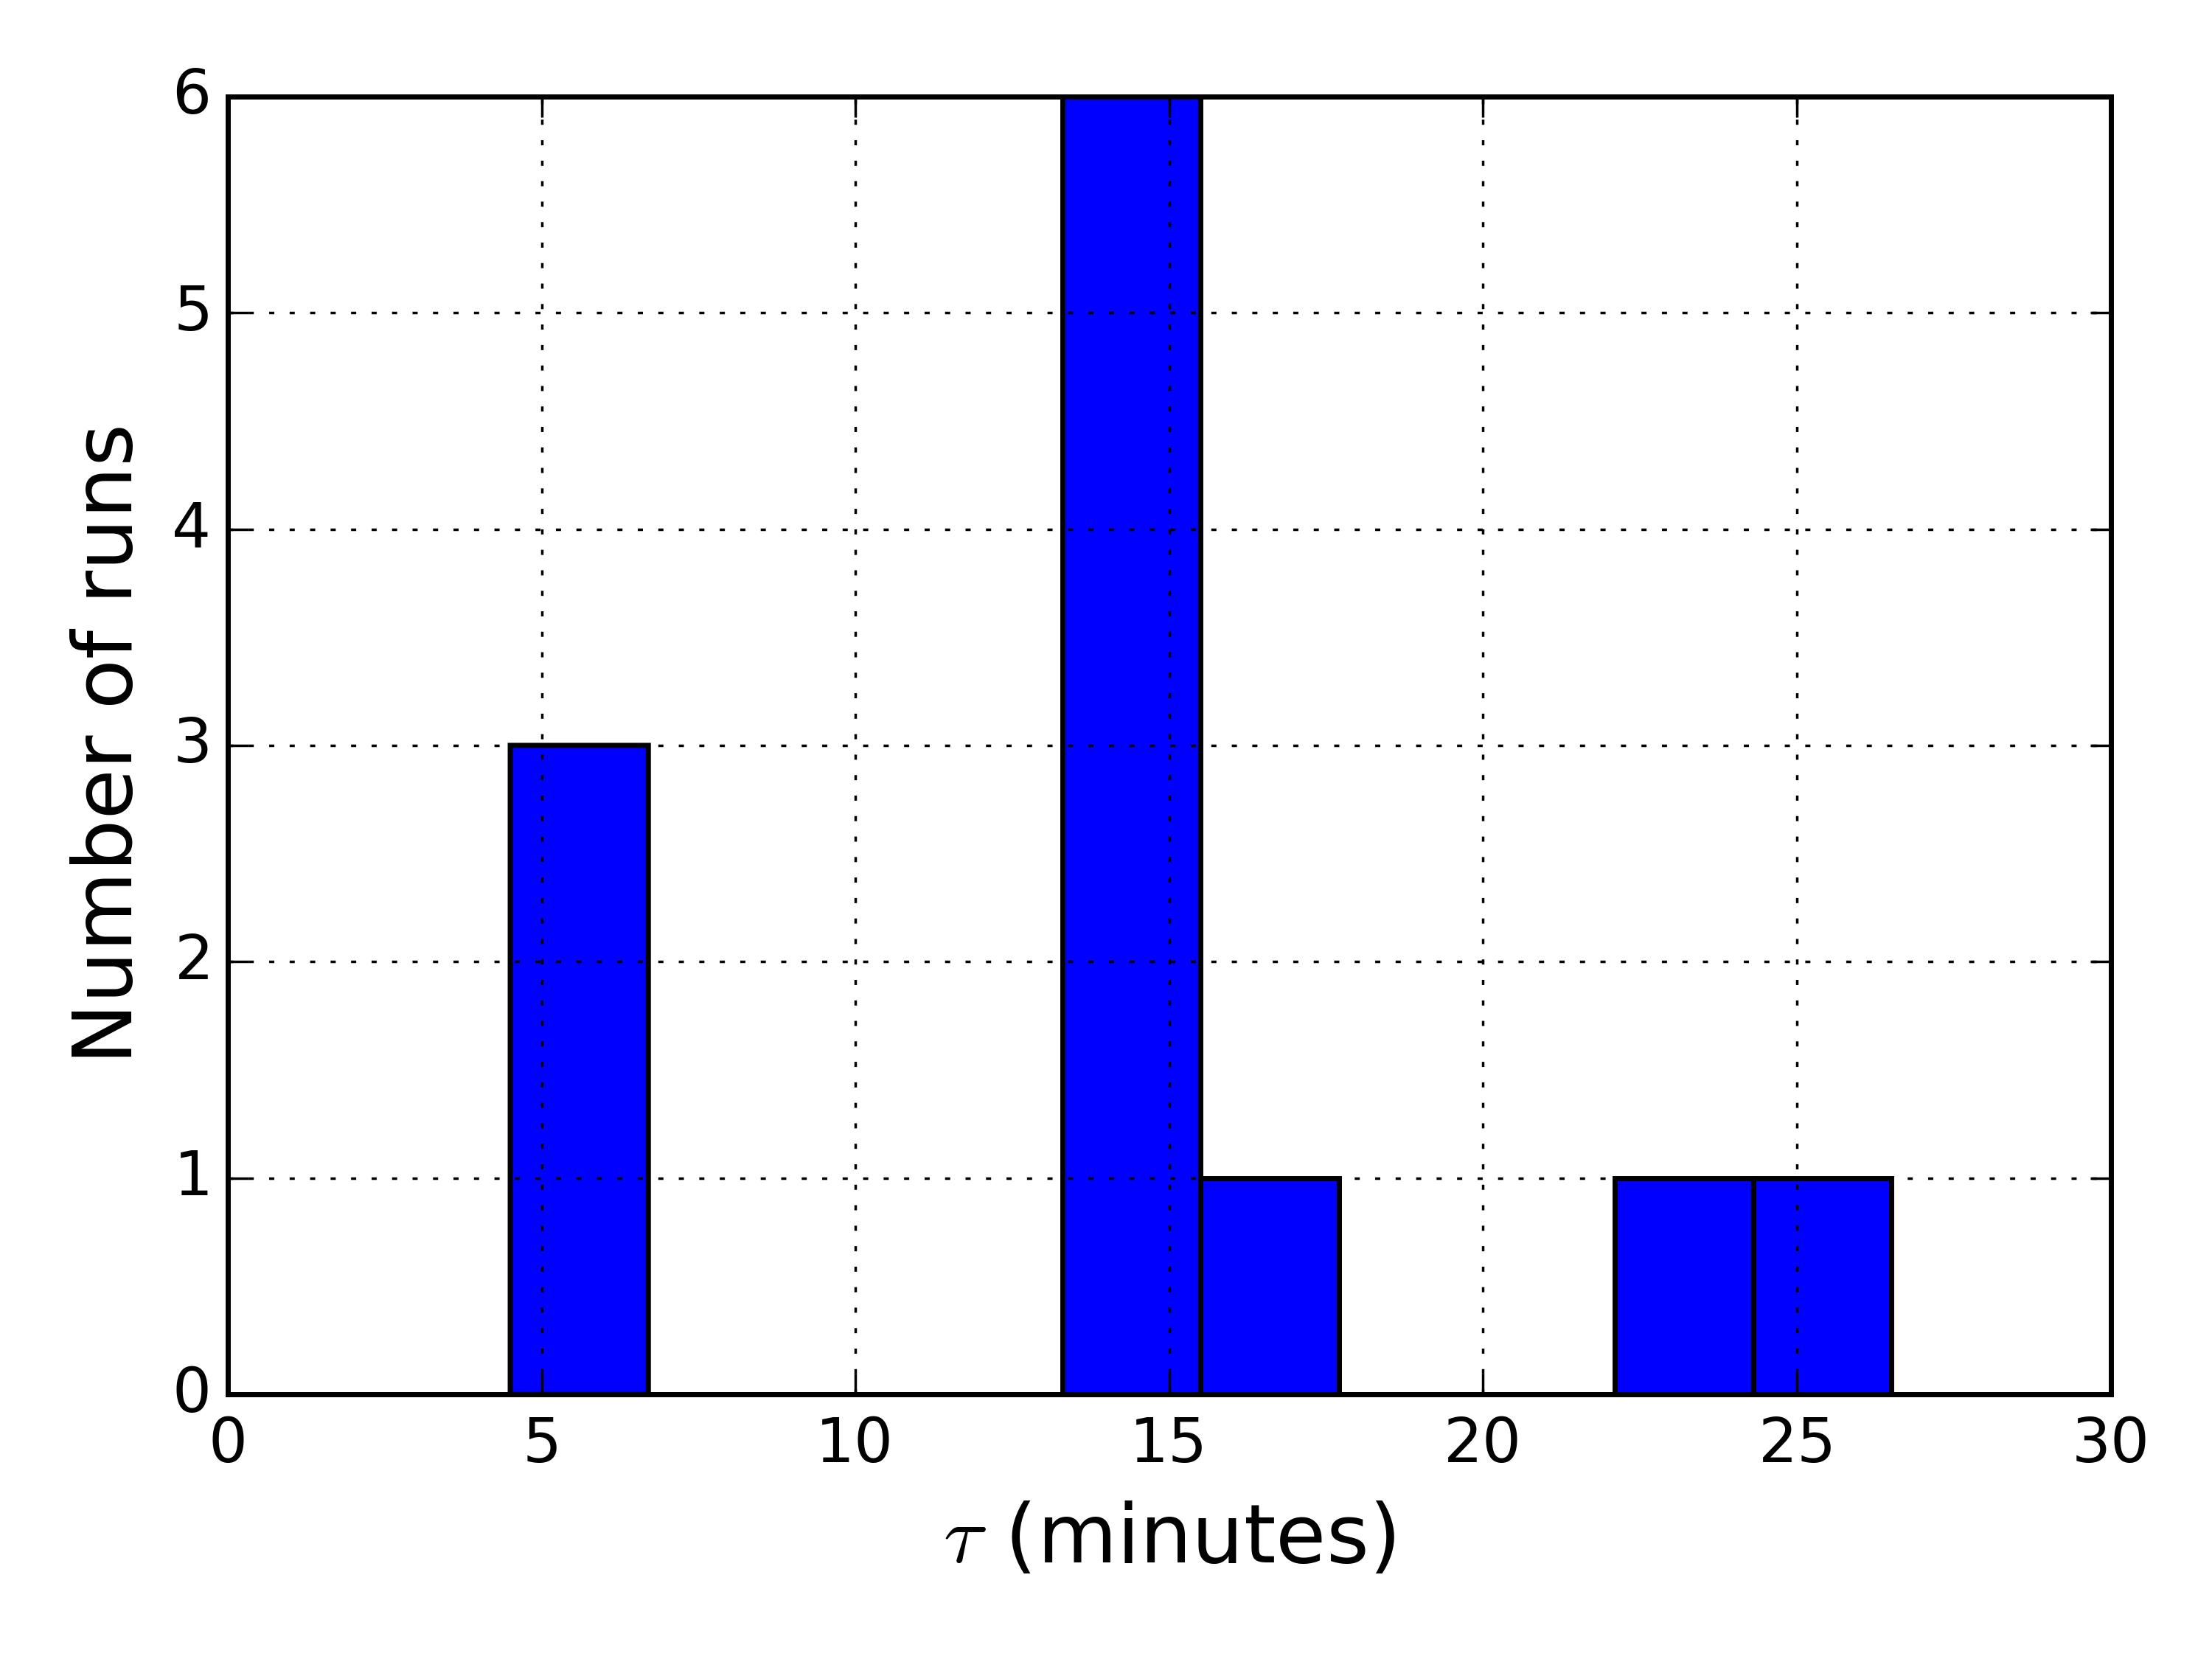
\includegraphics[width=0.5\textwidth]{FIGURES/hist.png}
\caption{histograms
\label{fig:hist}}
\end{figure}


Following~\cite{Racine1996}, we also define the structure-function-like quantity
\begin{equation}
       f(\Delta t) = {| \theta(t+\Delta t) - \theta(t)| \over  \theta(t+\Delta t) + \theta(t) },
\end{equation} 
where $\theta$ is seeing.
We then fit the mean value of $f(\Delta t)$ to 
\begin{equation}
    < f(\Delta t) > =  f(\Delta t) ^\infty \, \left[ 1 - \exp(-\Delta t/\tau)^\gamma \right],
\end{equation} 
The timescale $\tau$ is found to be mostly within the range of 15 $-$
25 minutes.



